\documentclass[11pt,a4paper]{scrartcl}
%{{{ general stuff
\usepackage[a4paper,bindingoffset=0.2in,%
            left=1in,right=1in,top=1in,bottom=1in,%
            footskip=.25in]{geometry}
\usepackage[english]{babel}
\usepackage[utf8]{inputenc}
\usepackage[T1]{fontenc}
\usepackage{cite}
\usepackage[hidelinks]{hyperref}
\usepackage{float} % use H in figure placement
\pagenumbering{gobble}

%}}}
%{{{ graphics
\usepackage{graphicx} % Bilder
%}}}
%{{{ math
\usepackage{mathrsfs} % mathcal and mathscr
\usepackage{mathtools, amssymb, amsthm}
\usepackage{bm} % cool bold symbols
%}}}

% a todo command===============================================================
\newcounter{todocounter}
\newcommand{\todo}[2][noisnotdefined]{
 \marginpar{\fcolorbox{black}{yellow}{\footnotesize\textbf{todo}}
 \ifthenelse{\equal{#1}{noisnotdefined}}{}{\textcolor{black}{\newline\tiny #1}}}
 \textbf{\ifthenelse{\equal{#2}{.}}
   {\fcolorbox{blue}{white}{\textcolor{blue}{$\maltese$}}}{{\textcolor{blue}{#2}}}}
 \refstepcounter{todocounter}}

%===============================================================================

\date{}
\title{Project Proposal for Genetic Algorithms and Evolutionary Programming}
\author{Felix Bartel and D\'avid Kerekes}

\begin{document}

\maketitle

\section{Problem Overview}

We want to apply a genetic algorithm to a neural network which is known as neuroevolution.
A big advantage of this scheme is that one only needs an indicator how good the neural network is given a certain task.
This can for instance be given by the outcome of a game.
Our game of choice was Blobby Volley 2 which is a simple two-dimensional volleyball game with open source written in C++ with lua support, see Figure \ref{fig:screenshot}.

\begin{figure}[H]
\center
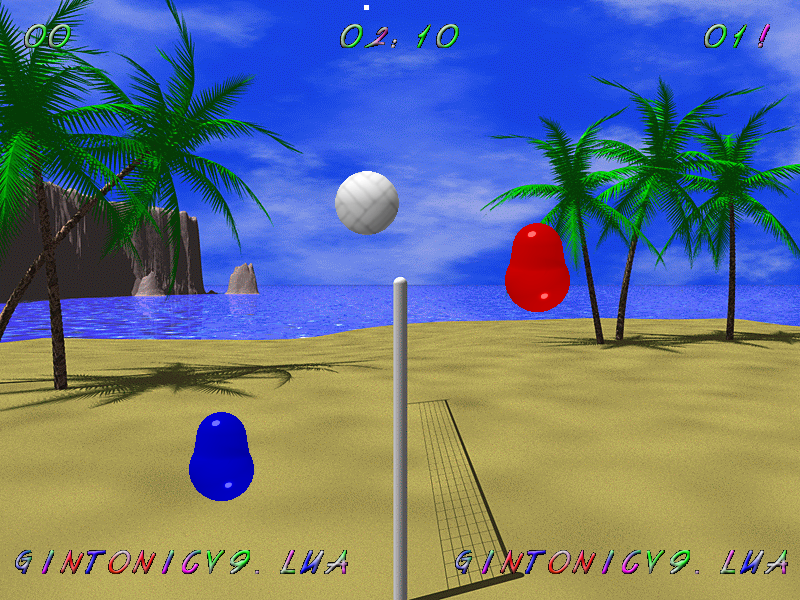
\includegraphics[width=0.7\textwidth]{img/screenshot.png}
\caption{Screenshot of the game.}
\label{fig:screenshot}
\end{figure}

A scene from the game could be described by the $x$- and $y$-coordinates of the players and the ball, their corresponding velocities and the current number of ball contacts.
These arguments or a subset of them could then be used as input for the neural network.
The output would then be the players movement which only consists of going right, left or jumping.
Assuming the layers of the neural network have $n_1,\dots,n_L$ nodes we then have to optimize \[N = \sum_{l=1}^{L-1} (n_l+1) \, n_{l+1}\] number of variables if we fix the size of the network.

\section*{Preliminary Results}

We have done some tests so far with a basic evolutionary algorithm \cite{github_repo} where we fixed the size of the neural network to $6$ input nodes, one hidden layer with $7$ nodes and $2$ output nodes.
As crossover we randomly mixed the weights and biases of two networks and chose the parents via the fitness proportional roulette wheel selection.
Mutation is accomplished by adding Gaussian noise to a subset of the nodes.
Furthermore we implemented elitism.


The representation of the network is accomplished through python objects. This will allow a straightforward implementation of a wide variety of genetic operators, while having next to no impact on the speed of training.
Evaluation of the population is done in a thread-parallel fashion, allowing us to exploit multiple high core-count machines at our disposal.

We implemented our own bot to act as an initial trainer for the network. This trainer is easier to defeat and even gives up after a certain amount of touches with the ball, such that normal gameplay will be rewarded.
The simplification gives the evolutionary algorithm the opportunity to start optimizing the neural network in a valid direction, without introducing additional factors to the fitness score.

\begin{figure}[H]
\center
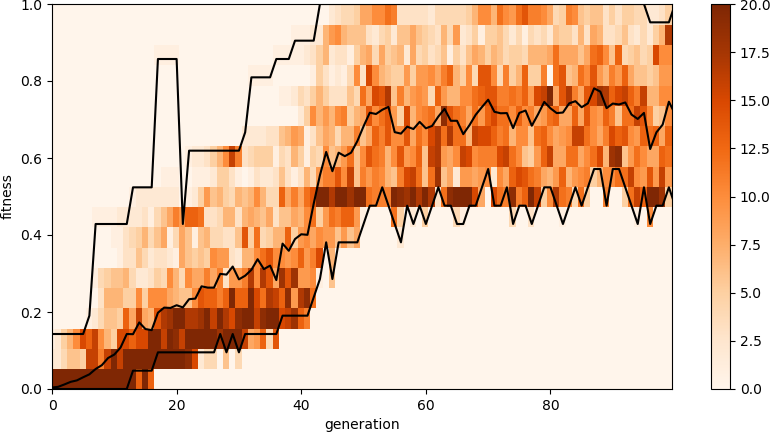
\includegraphics[width=0.9\textwidth]{img/fitness.png}
\caption{Fitness density of an example run with indicated minimum, average and maximum.}
\label{fig:train}
\end{figure}

The results are depicted in Figure \ref{fig:train}, where the fitness is the normalized point difference after $21$ serves.
One can see that, although we we made simplifications by weakening the opponent, the algorithm produces a network which wins all rounds.

\section*{Further Experiments}

We plan on testing multiple types of crossover and mutation operators, and selection schemes as seen in \cite{montana1989training}. Examples mutations include biased and unbiased weight mutations and node mutations. Example crossovers are weight, node, and feature crossovers.

To have a more objective representation of the capabilities of the networks, we plan on reintroducing the original easy, medium and hard difficulty bots in a curriculum-learning fashion.

Finally, as time allows we could extend this work by e.g.\,making the size of the network variable or do self-training with similar techniques as in the paper of Karl Sims\cite{sims1994evolving} presented in the lectures.

\bibliography{refs}{}
\bibliographystyle{plain}

\end{document}
